% !TeX spellcheck = en_US

\chapter{Related Work}
This chapter elaborates on the base technologies necessary to understand the following chapters.



\section{Geographic Information System (GIS)}
GIS contains of numerous technologies to store, manipulate, analyze and visualize geographical data. It can be used in all areas, that need to visualize spatial data. Some usages are: land-use, elevation data, weather maps, street networks and flood maps. To leverage the capabilities that GIS offers it is necessary to use specialized GIS software.


\subsection{Coordinate Reference System (CRS)}
In comparison to normal image data, GIS is always geo-referenced. This is achieved by specific geo-aware formats that encode spatial positions into the data. \\
When displaying GIS, it is almost always necessary to project the round shape of earth onto a plane. This process transfers the data to a so called \enquote{spatial reference system} (SRS) or \enquote{coordinate reference system} CRS.\\
Depending on the area of earth, different projections result in optimal results. Some are optimized for certain areas, while others offer an acceptable worldwide view. Figure \ref{fig:mercator} shows the Mercator projection in it's normal and transverse orientation, which focuses on the poles. The normal orientation is used by maps like OpenStreetMap (OSM), google maps and the Global Positioning System (GPS).\\
The normal Mercator projection may also be referred to as \enquote{World Geodetic System 1984} (WGS 84). Several standards by the \enquote{European Petroleum Survey Group}  (EPSG) exist. The two most common are EPSG:4326 which is a geographic coordinate system used for GIS files, OSM data and Google earth. EPSG:3857 is a projected coordinate system and is used by the OSM WebMapService (WMS) as well as Google Maps.
\begin{figure}[H]
	\centering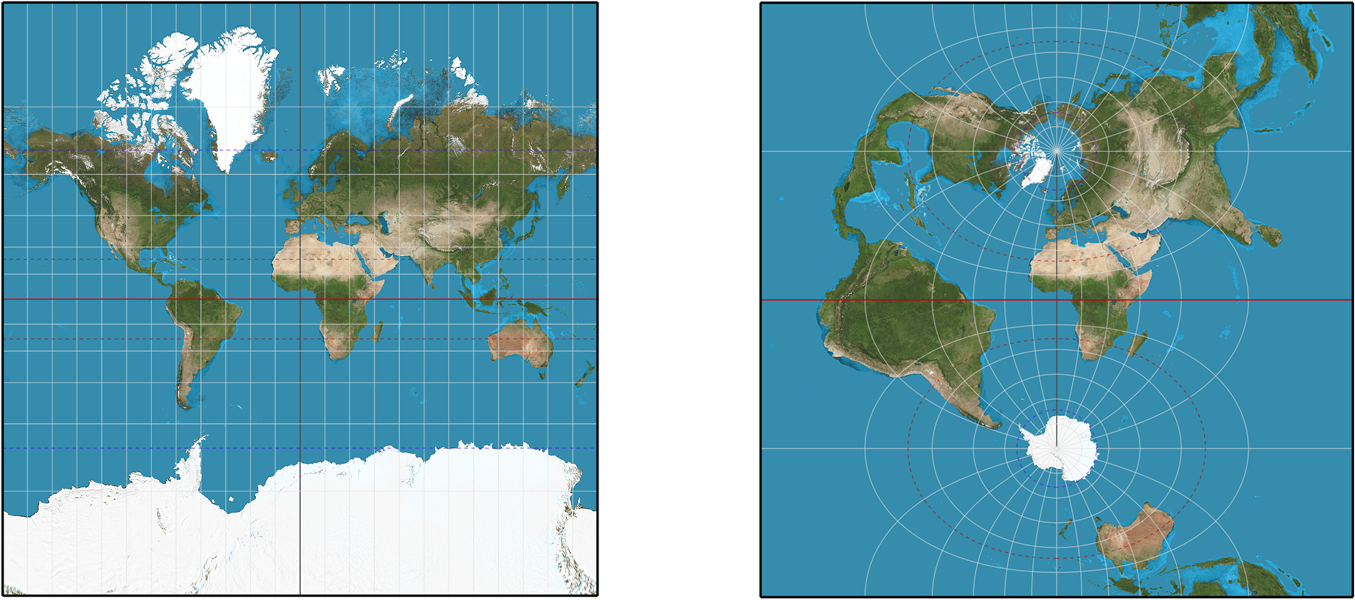
\includegraphics[width=1\textwidth]{res/Mercator}
	\caption{Normal and transverse Mercator projection by Peter Mercator. \url{https://commons.wikimedia.org/w/index.php?curid=9910866}}
	\label{fig:mercator}
\end{figure}


\subsection{File Types}
GIS files exist in two different types, vector and raster. 

\subsubsection{Raster Data}
 Raster data consists of a grid that is filled with color values. Each pixel stores information as a numeric value. These values can be numeric (e.g. for an elevation map) as well as encoded grayscale or color values.\\
 The advantage of raster data is that it can store any kind of GIS. the disadvantages are big files and the fixed pixel resolution.

\subsubsection{Vector Data}
Vector GIS on the other hand has a much smaller file size, but is limited in its capabilities. It stores information based on mathematical functions. While this is very efficient, it is not suited for image like data such as land-use or elevation maps.\\
Data inside vector GIS is called a feature. Features are composed of either points, polylines or polygons. It is well suited to store data such as hot-spots, borders, contour lines, etc. Figure \ref{fig:vector-raster} shows a shape as a vector and in three different raster resolutions.
\begin{figure}[H]
	\centering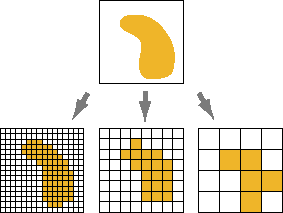
\includegraphics[width=.5\textwidth]{res/Vector-Raster}
	\caption{Vector as raster in different resolutions. \url{http://desktop.arcgis.com/en/arcmap/latest/manage-data/raster-and-images/what-is-raster-data.htm}}
	\label{fig:vector-raster}
\end{figure}



%\section{Mono}
%Open C\# implementation for Linux and OSX.
%
%
%
%\section{.NET Core}
%Microsoft bought Xamarin, which mostly developed Mono and is creating it's new C\# with build in multi-platform support.